%======================================================================
\section{Numerical tests}\label{sec:num}
%======================================================================

\subsection{Methods}\label{sec:num-methods}

\paragraph{Simulation.} States are stabilizer states, stored in a transposed, pre-allocated tableau whose generators are packed in 64-bit words \cite{AaronsonGottesman2004}. The entropy of a region is computed exactly as a rank over $\mathbb F_2$ \cite{Fattal2004}; for a stabilizer state the entanglement spectrum is flat, $S=S_2=S_\infty$. The strict cone $\Inf(A)$ is computed exactly by the backward sweep, with every gate recorded. Haar circuits ($q=2$, $N\le22$) are simulated as state vectors, and $S$ and $S_2$ are obtained from the Schmidt decomposition.

\paragraph{Gates.} The two-qubit Clifford group modulo Paulis is $\mathrm{Sp}(4,\mathbb F_2)$, of order $720$. Signs do not affect any entropy, so drawing the symplectic part uniformly reproduces the law of entropies under the uniform Clifford group, which is a 2-design \cite{DLT2002,Webb2016,Zhu2017}. We enumerated the $720$ matrices and checked closure of the group. The uniform Clifford group is even a 3-design \cite{Webb2016,Zhu2017}: the annealed averages of Theorems~D and~E are \emph{exactly} those of Haar; what can differ are quenched averages and the von Neumann entropy (Section~\ref{sec:num-haar}). One pitfall is worth reporting. The ensemble obtained by composing three layers of uniform elements of $\mathrm{SL}(2,\mathbb F_2)$ separated by two opposite CNOTs (``rand2'') reaches only $684$ of the $720$ elements, with multiplicities from $64$ to $144$ over the $6^6$ combinations: it is not a 2-design, and the purity test below rejects it. All values reported in this paper use uniform gates.

\paragraph{Statistics.} Averages are over independent circuits whose seeds are fixed in the scripts (Appendix~\ref{app:repro}). The standard error, given in parentheses on the last digits or after $\pm$, is the sample standard deviation (with Bessel's correction) divided by $\sqrt n$; the number $n$ of seeds is given in each caption. Slopes $dG/dN$ are fitted by least squares on each seed and then averaged; their standard error is that of the slopes between seeds. The exponents of Table~\ref{tab:2d} are log-log slopes between two sizes, computed on the means; their standard error is estimated by a bootstrap over seeds ($10^4$ resamplings). The lower (cone) and upper (annealed recursion) bounds at finite size are exact, so when a mean is compared with one of them the quoted uncertainty is purely statistical. Systematic uncertainties are finite-size effects: we do not extrapolate in $N$ except where the exact finite-size bound is available.

\paragraph{Pre-registration.} Every campaign was preceded by written, time-stamped predictions with success criteria (folder \texttt{preregistration/} of the repository). Predictions that failed are reported where they occur: the velocity threshold (Section~\ref{sec:num-edge}), two quantitative values for $N\propto t$ and the fast exponential front (Sections~\ref{sec:num-1d} and~\ref{sec:num-2d}), the agreement criterion between Haar and Clifford (Section~\ref{sec:num-haar}), the parity criterion at four seeds (Section~\ref{sec:num-1d}), one criterion for correlated births (Section~\ref{sec:num-correlated}) and one criterion of the free-field test (Section~\ref{sec:energy}). The repository's \texttt{preregistration/README.md} lists every prediction with its outcome.

\subsection{Checks of the 2-design and of the wall model}\label{sec:num-checks}

\emph{Single-wall recursion against the full model.} The recursion of Proposition~\ref{prop:single} was compared with an exact computation of the full spin model in the output gauge, which sums over the $3^n$ states with no assumption on walls. Over $18$ geometries ($q=2,3$; $N_0=2,\dots,5$; $n\le12$; $k=1,\dots,4$) and all cuts, the maximal relative deviation is $3.4\times10^{-15}$.

\emph{Uniform Clifford against the exact value.} For each of $9$ geometries, $2\times10^5$ circuits were drawn. The mean purity $\E[2^{-S(A)}]$ agrees with the exact $Z_A$ within $|z|\le2.3$. With rand2, the deviation is $z=+75$ to $+211$, the purity being $8$ to $54\,\%$ too high. The same check for Haar gates is reported in Table~\ref{tab:haar}.

\emph{Velocities.} The measured butterfly velocity (front of a Pauli operator, $200$ seeds) is $v_B=0.6004(42)$, against exactly $0.6$ for a 2-design \cite{NVH2018}. The quenched entanglement velocity, measured on a fixed chain of $512$ qubits with $8$ seeds, is $v_E=0.323(5)$ to $0.328(3)$ bit per layer depending on the fit window, just above the annealed value $v_E^{(2)}=0.3219$, which bounds it from below for every 2-design (Jensen's inequality, since $S=S_2$ for stabilizer states).

\emph{Theorem A.} No violation appears in $5632$ exact checks: $2400$ random Clifford circuits on random graphs with births, $2700$ Haar circuits with insertion, and $532$ checkpoints of the 1D and 2D campaigns of Sections~\ref{sec:num-1d} and~\ref{sec:num-2d}. The $261\,450$ circuits of Table~\ref{tab:haar} ($21\,450$ Haar, $240\,000$ Clifford) also satisfy it.

\subsection{Edge growth: no threshold, and the bracket}\label{sec:num-edge}

\begin{table}[h]
\centering\small\setlength{\tabcolsep}{4pt}
\begin{tabular}{rcccccc}
\toprule
$k$ & lower bound & uniform Clifford & upper bound & $\frac{\text{upper}-\E[G]}{\text{upper}}$ & Theorem E & membrane estimate\\
 & (cone, finite $m$) & $\E[G]/N$ & (recursion, finite $m$) & ($\%$) & $m\to\infty$ & $\frac12\max(1-kv_E,\frac{1}{1+kv_B})$\\
\midrule
1  & 0.2500 & 0.3516 (10) & 0.3538 & $+0.60\,(27)$ & 0.354 & 0.338\\
2  & 0.1665 & 0.2566 (5) & 0.2578 & $+0.46\,(18)$ & 0.258 & 0.227\\
4  & 0.0996 & 0.1616 (6) & 0.1618 & $+0.13\,(36)$ & 0.162 & 0.147\\
8  & 0.0552 & 0.0902 (2) & 0.0914 & $+1.38\,(18)$ & 0.092 & 0.086\\
16 & 0.0293 & 0.0487 (5) & 0.0484 & $-0.53\,(96)$ & 0.049 & 0.047\\
32 & 0.0146 & 0.0244 (0)$^\ast$ & 0.0248 & $+1.47$ & 0.025 & 0.025\\
\bottomrule
\end{tabular}
\caption{Edge growth, in bits per degree of freedom. Uniform Clifford: $N=2048$ and $6$ seeds for $k\le8$; $N=1024$ and $6$ seeds for $k=16$ and $32$. The lower and upper bounds are computed exactly at the same size; the column ``Theorem E'' gives the limit of the upper bound as $m\to\infty$. The membrane estimate, which is not a bound, uses $v_E=0.325$ and $v_B=0.6$. $^\ast$All six seeds give the same entropy ($487$ bits); the standard error is below $10^{-4}$.}
\label{tab:edge}
\end{table}

\begin{figure}[t]
\centering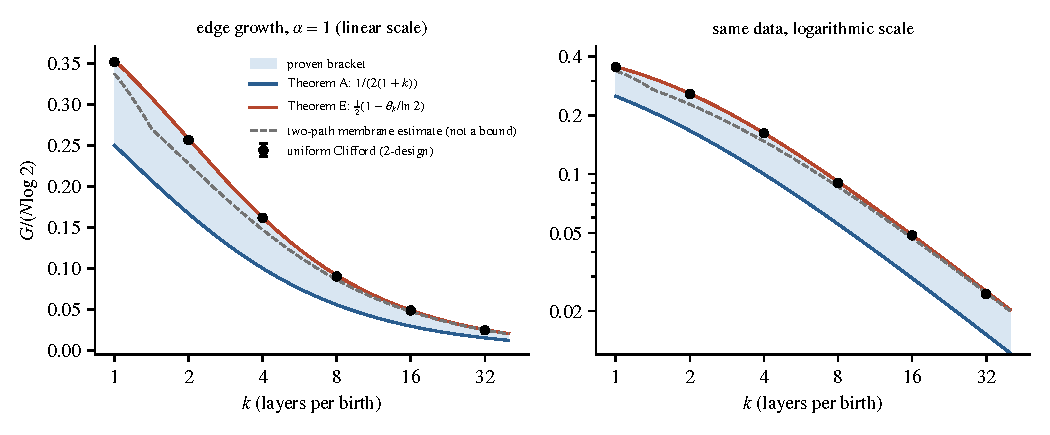
\includegraphics[width=\textwidth]{figures/fig_edge.pdf}
\caption{Edge growth ($\alpha=1$). The blue band is the proven bracket (Corollary~\ref{cor:bracket}). Black points: uniform Clifford circuits. Dashed: two-path membrane estimate. The deficit stays extensive for every $k$: the threshold prediction registered at the start, $k\,v_E\gtrsim\frac12$, is refuted.}
\label{fig:edge}
\end{figure}

Three observations stand out (Table~\ref{tab:edge}, Figure~\ref{fig:edge}).
(i)~There is no threshold: $G/N$ decreases like $1/k$ without ever vanishing, including when $kv_E$ is well above $\frac12$. The threshold prediction registered at the start is refuted.
(ii)~All values respect the proven bracket. Compared with the upper bound evaluated at the same size, they lie $0.13$ to $1.5\,\%$ below it; at $k=16$ the value exceeds the bound by $0.5\,\%$, i.e.\ $0.6$ standard error, which is compatible with Jensen's inequality. Equivalently, the quenched entropy density $\E[S]/m$ exceeds the exact annealed density by $0.0042(19)$, $0.0024(9)$, $0.0004(12)$ and $0.0025(3)$ bit per qudit for $k=1,2,4,8$ ($m=1024$); for $k=16$ and $32$ the difference is below $0.001$ bit.
(iii)~The two-path membrane estimate, which is not a bound, stays $3$ to $11\,\%$ below the data for $k\le16$ and exceeds them by $1.4\,\%$ at $k=32$. Theorem~E replaces it by a proven bound.
Stabilizer states have a flat entanglement spectrum ($S=S_2$); the next subsection compares with Haar gates at small sizes.

\subsection{Haar against Clifford at equal size}\label{sec:num-haar}

The uniform Clifford group gives exactly the annealed averages of Haar, but not necessarily the quenched ones, and its states have a flat entanglement spectrum. To separate these two effects, we simulated Haar circuits as state vectors in the exact geometry of Theorems~D and~E (edge growth, $N_0=2$, $A=[0,m)$, $N=2m$), and Clifford circuits in the same geometries (Table~\ref{tab:haar}). The predictions were written before the code.

\begin{table}[h]
\centering\footnotesize\setlength{\tabcolsep}{3.2pt}
\resizebox{\textwidth}{!}{%
\begin{tabular}{rrccccccccc}
\toprule
$N$ & $k$ & lower bound & Haar, $m-\E[S]$ & Clifford, $m-\E[S]$ & Haar, $m-\E[S_2]$ & upper bound & position $\varrho$ & $\E[S-S_2]$ (Haar) & annealed $z$\\
\midrule
12 & 1 & 3 & 3.904\,(3) & 4.101\,(5) & 4.251\,(4) & 4.274 & 0.71 / 0.86 / 0.98 & 0.347 & $-0.7$ / $+1.2$ \\
12 & 2 & 2 & 2.692\,(2) & 2.875\,(5) & 3.050\,(3) & 3.062 & 0.65 / 0.82 / 0.99 & 0.357 & $-0.3$ / $0.0$ \\
12 & 4 & 1 & 1.725\,(2) & 1.888\,(5) & 2.064\,(2) & 2.071 & 0.68 / 0.83 / 0.99 & 0.339 & $-1.8$ / $-1.1$ \\
16 & 1 & 4 & 5.223\,(5) & 5.454\,(5) & 5.644\,(6) & 5.673 & 0.73 / 0.87 / 0.98 & 0.422 & $-1.1$ / $-1.4$ \\
16 & 2 & 2 & 3.528\,(4) & 3.774\,(6) & 3.987\,(4) & 4.003 & 0.76 / 0.89 / 0.99 & 0.459 & $-0.5$ / $+0.2$ \\
16 & 4 & 1 & 2.200\,(3) & 2.398\,(5) & 2.567\,(3) & 2.576 & 0.76 / 0.89 / 0.99 & 0.366 & $-1.5$ / $+0.6$ \\
20 & 1 & 5 & 6.573\,(7) & 6.838\,(6) & 7.061\,(8) & 7.080 & 0.76 / 0.88 / 0.99 & 0.487 & $+0.2$ / $+0.8$ \\
20 & 2 & 3 & 4.508\,(6) & 4.760\,(6) & 4.992\,(6) & 5.006 & 0.75 / 0.88 / 0.99 & 0.484 & $-0.2$ / $+0.1$ \\
20 & 4 & 2 & 2.745\,(3) & 2.928\,(5) & 3.121\,(4) & 3.124 & 0.66 / 0.83 / 1.00 & 0.376 & $+0.6$ / $+0.2$ \\
22 & 1 & 6 & 7.556\,(18) & 7.834\,(6) & 8.046\,(21) & 8.078 & 0.75 / 0.88 / 0.98 & 0.489 & $-0.4$ / $+0.3$ \\
22 & 2 & 4 & 5.219\,(15) & 5.487\,(6) & 5.720\,(17) & 5.741 & 0.70 / 0.85 / 0.99 & 0.501 & $-0.4$ / $-1.0$ \\
22 & 4 & 2 & 3.140\,(11) & 3.352\,(5) & 3.558\,(12) & 3.561 & 0.73 / 0.87 / 1.00 & 0.418 & $+0.4$ / $-0.8$ \\
\bottomrule
\end{tabular}}
\caption{Mean deficit (bits) in the geometry of Theorems~D and~E, $q=2$. Haar: $4000$, $2000$, $1000$ and $150$ circuits for $N=12$, $16$, $20$ and $22$; Clifford: $2\times10^4$ circuits per geometry. Lower (cone) and upper ($m+\log_2Z_A$) bounds are exact. Position $\varrho=(\E[G]-\text{lower})/(\text{upper}-\text{lower})$ for Haar--von Neumann, Clifford and Haar--R\'enyi-2. $z$: deviation of $\E[2^{-S_2}]$ from the exact $Z_A$, in standard errors, for Haar and Clifford.}
\label{tab:haar}
\end{table}

\begin{itemize}[leftmargin=*,itemsep=1pt]
\item \emph{Checks.} The mean purity agrees with the exact $Z_A$ in every geometry ($|z|\le1.8$). No circuit violates Theorem~A.
\item \emph{Ordering.} In every geometry, $\E[G]$ for Haar--von Neumann $<$ $\E[G]$ for Clifford $<$ $m-\E[S_2]$ for Haar $\le$ upper bound. The positions inside the bracket are $0.65$--$0.76$ (Haar, von Neumann), $0.82$--$0.89$ (Clifford) and $0.98$--$1.00$ (Haar, R\'enyi-2).
\item \emph{Haar R\'enyi-2.} The quenched mean $\E[S_2]$ exceeds the annealed value by only $0.003$ to $0.032$ bit: for Haar, Jensen's inequality $\E[S_2]\ge\Srec$ is nearly saturated, and Theorem~E predicts the quenched R\'enyi-2 entropy to this accuracy.
\item \emph{Haar von Neumann.} The difference $D(m)=\E[S]-\E[S_2]$ is $0.34$ to $0.50$ bit. It grows with $m$, but more and more slowly for $k=1$ ($0.35$, $0.42$, $0.49$, $0.49$ bit at $N=12$, $16$, $20$, $22$); for $k=4$ it keeps growing ($0.38$ then $0.42$ bit at $N=20$ and $22$). Weighted fits of $D(m)$ by $a+bm$, $a+b\ln m$ and $a-b/m$ (\texttt{haar\_vs\_clifford\_analysis.py}) are all poor, with $\chi^2\ge21$ for $2$ degrees of freedom for every $k$; the last point ($m=11$) is the only odd $m$, and parity effects of the kind seen in Remark~\ref{rem:finitesize} are a plausible cause. The data therefore do not discriminate between a bounded $D(m)$ and one that grows linearly with a small slope, which is what the theory of random circuits suggests (see below).
\item \emph{Clifford} is intermediate: its entropy, equal to its R\'enyi-2 entropy, exceeds the quenched Haar R\'enyi-2 entropy by $0.15$ to $0.23$ bit, a difference that varies little between $N=20$ and $22$.
\item \emph{Pre-registration.} Four criteria are confirmed (annealed check; $\E[S]>\E[S_2]$ and growth with $m$; ordering Haar--von Neumann $<$ Clifford; higher position for Clifford). The criterion $|\E[S_2]_{\rm Haar}-\E[S]_{\rm Clifford}|\le0.2$ bit \emph{fails} from $N=16$ on, with at most $0.23$ bit.
\end{itemize}
At these sizes the width of the bracket (about two bits) is comparable to the differences between ensembles, so the position $\varrho$ depends on the ensemble and on the entropy chosen. Densities are another matter, and the two entropies should be treated separately. For R\'enyi-2, the quenched--annealed difference is expected to be small: in random circuits of fixed size it comes from interactions between replicas and is parametrically small at large $q$ \cite{ZhouNahum2019}, in agreement with the $0.003$ to $0.032$ bit observed here and with the Clifford data at large size. For the von Neumann entropy there is no such expectation. At finite $q$ the entanglement velocity, and more generally the line tension, depends on the R\'enyi index, and the dependence disappears only as $q\to\infty$ \cite{ZhouNahum2019}. Transposed to Theorem~E, whose density $\theta_k$ is the minimal cost of a wall ending on the line of births, this suggests (heuristically) that at $q=2$ the von Neumann density differs from the annealed R\'enyi-2 density by an amount of order one per site, i.e.\ that $D(m)$ grows linearly in $m$ with a small slope; the data (linear slopes $0.03$ bit per site for $k=1,2$ and $0.01$ for $k=4$, with poor fits) neither confirm nor exclude this. What is proven is unaffected: since $S\ge S_2$, the bracket of Corollary~\ref{cor:bracket} holds for the von Neumann entropy, and only the position inside it is open. What is established numerically is that the annealed bound predicts the quenched Haar R\'enyi-2 entropy to a few hundredths of a bit, and R\'enyi-2 is the quantity estimated by randomised-measurement protocols \cite{Brydges2019}.

\subsection{Births in pairs}\label{sec:num-pairs}

\begin{table}[h]
\centering\small
\begin{tabular}{rccccc}
\toprule
$k$ & R (pure qudit) & P1 (local pair) & P2 (non-local pair) & R/P2 & R/P2, minimal cut\\
\midrule
0  & 0.5000 & 0.5000 & 0.2486 (72) & 2.01 (6) & 2\\
1  & 0.3515 (11) & 0.3521 (6) & 0.1575 (53) & 2.23 (8) & 2.05\\
2  & 0.2559 (8) & 0.2565 (5) & 0.0874 (61) & 2.93 (20) & 2.76\\
4  & 0.1600 (4) & 0.1614 (7) & 0.0459 (27) & 3.49 (20) & 3.09\\
8  & 0.0912 (3) & 0.0911 (2) & 0.0268 (20) & 3.40 (25) & 3.09\\
16 & 0.0483 (2) & 0.0484 (4) & 0.0134 (12) & 3.61 (33) & 4.12\\
32 & 0.0252 (3) & 0.0249 (1) & 0.0051 (8) & 4.90 (74) & ---\\
\bottomrule
\end{tabular}
\caption{Slope $dG/dN$ (bit per degree of freedom), fitted on $N\in[200,800]$, uniform Clifford, $8$ seeds, edge growth. Scrambling is $k$ layers per added degree of freedom in all three variants. Last column: the same ratio for the exact minimal cut of the space-time network ($n\le160$, $3$ seeds; the value at $k=0$ is exact).}
\label{tab:pairs}
\end{table}

Suppose each distinction creates a Bell pair; there are two cases (Table~\ref{tab:pairs}).
\emph{Local pair (P1).} The slope is indistinguishable from the reference for every $k$, within $1.7$ standard errors. The birth condition does not require each degree of freedom to be born pure; it requires it to be born without \emph{long-range} correlation with the pre-existing world (Remark~\ref{rem:pairs} and Section~\ref{sec:num-correlated}).
\emph{Non-local pair (P2):} one member is born at the edge, the other inserted at a uniformly random position. Without scrambling ($k=0$), the added deficit is $\frac14$ per degree of freedom instead of $\frac12$, because one pair in two straddles the cut. With scrambling, the weakening R/P2 goes from $2.2$ to $3.6$ for $k=1,\dots,16$, and is $4.9\pm0.7$ at $k=32$; this last value lies outside the announced interval $[2,4.5]$ while remaining compatible with it within one standard error. The slope stays positive: the arrow is weakened, not erased. An exact minimal cut of the space-time network, in which each Bell pair is a link that the cut must cross (\texttt{mincut\_pairs.py}), gives ratios of $2.05$ to $4.12$ for $k=1,\dots,16$, within about $15\,\%$ of the measured ones, but at smaller sizes ($n\le160$). The geometry of the shortcuts thus accounts for the order of magnitude of the effect; the residual differences, of either sign, are not explained here.

\subsection{Births correlated with the past}\label{sec:num-correlated}

\begin{table}[h]
\centering\small\setlength{\tabcolsep}{5pt}
\begin{tabular}{lcccccc}
\toprule
 & $f=0$ & $0.01$ & $0.03$ & $0.1$ & $0.3$ & $1$\\
\midrule
$k=1$, non-local & 0.3518 (5) & 0.3485 (14) & 0.3435 (14) & 0.3332 (45) & 0.2828 (44) & 0.1415 (40)\\
$k=1$, local & & & & 0.3514 (7) & & 0.3521 (8)\\
$k=4$, non-local & 0.1597 (6) & 0.1602 (7) & 0.1575 (11) & 0.1521 (15) & 0.1264 (16) & 0.0604 (28)\\
$k=4$, local & & & & 0.1609 (4) & & 0.1612 (8)\\
\bottomrule
\end{tabular}
\caption{Slope $dG/dN$ (bit per degree of freedom) on $N\in[200,800]$, edge growth, uniform Clifford, $8$ seeds. With probability $f$, the newborn undergoes at birth a uniform Clifford gate with an existing site: its immediate neighbour (local) or an existing site drawn uniformly (non-local). The mean mutual information between the newborn and the past, just after a correlated birth, is $1.6$ bit (non-local) and $0.9$ to $1.6$ bit (local).}
\label{tab:correlated}
\end{table}

Table~\ref{tab:correlated} quantifies Proposition~\ref{prop:births}(c) and Remark~\ref{rem:pairs}.
\begin{itemize}[leftmargin=*,itemsep=1pt]
\item \emph{Local correlation:} even with $f=1$ and a mutual information of order one bit per birth, the slope does not change ($|\text{difference}|\le1.7$ standard errors). The amount of correlation with the past is not the relevant variable.
\item \emph{Non-local correlation:} the slope decreases with $f$. For $f\le0.1$, each correlated birth costs on average $0.2$ to $0.3$ bit of deficit for $k=1$ and about $0.08$ bit for $k=4$, less than the instantaneous bound $\frac12I\approx0.8$ bit of Proposition~\ref{prop:births}(c), which takes into account neither the position of the partner nor the subsequent scrambling. At $f=1$ the slope is divided by $2.5$ ($k=1$) and $2.6$ ($k=4$), but stays positive by more than $20$ standard errors: the arrow is weakened, not erased.
\item \emph{Pre-registration:} the announced criteria are met, except the relative reduction at $f=0.1$ for $k=4$, which is $4.8(10)\,\%$ for an announced interval $[5\,\%,75\,\%]$; the miss is smaller than one standard error.
\end{itemize}

\subsection{Annealed and quenched; the regime $\alpha<1$}\label{sec:num-alpha}

\begin{figure}[t]
\centering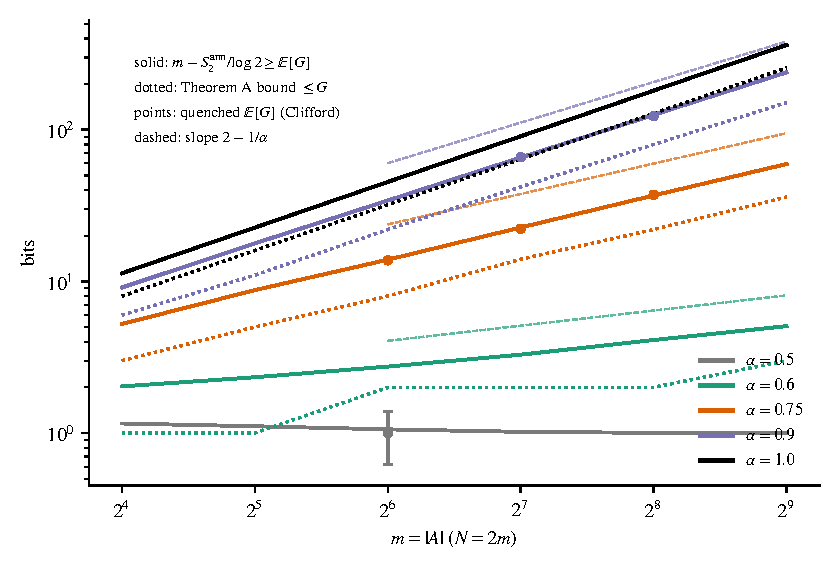
\includegraphics[width=0.72\textwidth]{figures/fig_alpha.pdf}
\caption{Growth $n-N_0=\lfloor L^\alpha\rfloor$. Solid: $m-\Srec/\log2$, an exact upper bound on $\E[G]$. Dotted: the lower bound of Theorem~A, valid for every circuit. Points: quenched $\E[G]$ for uniform Clifford circuits ($8$ seeds). Dashed: slope $2-1/\alpha$ of Corollary~\ref{cor:alpha}.}
\label{fig:alpha}
\end{figure}

\emph{Exact annealed density.} The exact recursion, computed in the log domain, gives $-\log_2 Z_A/m=0.29248$, $0.48428$, $0.67606$ and $0.81682$ for $k=1,2,4,8$ at $m=16\,384$. The agreement with $\theta_k/\ln2$ is within $0$ to $2\times10^{-5}$, and the correction $-\log Z_A-\theta_km$ converges to a constant, as Theorem~E predicts. At $k=1$, the ratio $Z_A\,(3/2)^{m/2}$ equals $1.000000$ for even $m$ from $m=40$ on, and $(3/2)^{\pm1/2}$ for odd $m$, depending on the phase (Proposition~\ref{prop:k1}).

\emph{Regime $\alpha<1$.} For $\alpha\in\{0.4,0.5,0.6,0.75,0.9,1\}$ and $m=16$ to $512$, with up to $10^6$ layers, the chain ``bound~A $\le m-\Srec/\log2\le B(t^\ast)+1.70$'' holds in all $34$ cases, with a minimal margin of $0.70$ bit (Figure~\ref{fig:alpha}). The log-log slopes over the three largest $m$ are $0.42$, $0.72$ and $0.94$ for $\alpha=0.6$, $0.75$ and $0.9$, against the proven asymptotic exponents $0.33$, $0.67$ and $0.89$; the difference is expected at these sizes. For $\alpha\le\frac12$, $m-\Srec/\log 2\to1$ bit. The quenched Clifford values ($8$ seeds) are $13.75(25)$, $22.25(25)$ and $37.25(37)$ bits for $\alpha=0.75$ and $m=64$, $128$, $256$, to be compared with the annealed bounds $13.90$, $22.67$ and $36.86$; the last point exceeds its bound by $1.1$ standard errors, which is compatible.

\subsection{Insertion in one dimension and parity locking}\label{sec:num-1d}

\begin{table}[h]
\centering\small
\begin{tabular}{lcccccc}
\toprule
growth & $G/N$ ($400$) & $G/N$ ($1600$) & $G_{\rm LB}/N$ ($1600$) & prediction ($v=1$) & with $v_{\rm eff}$ & $S$ ($1600$) \\
\midrule
edge, $k=1$ & $0.347$ & $0.3502\,(12)$ & $0.2500$ & $0.250$ & --- & $240\,(2)$ \\
edge, $k=4$ & $0.161$ & $0.1595\,(9)$ & $0.1000$ & $0.100$ & --- & $545\,(2)$ \\
$N\propto t^{1/2}$ & $0.015$ & $0.0033\,(4)$ & $0.0020\,(4)$ & $0.001$ & $0.001$ & $795\,(1)$ \\
$N\propto t$ & $0.411$ & $0.4155\,(15)$ & $0.2711\,(36)$ & $\mathbf{0.184}$ & $0.261$ & $135\,(2)$ \\
$N\propto t$, pairs & $0.341$ & $0.3381\,(11)$ & $0.1889\,(13)$ & $0.184$ & $0.184$ & $259\,(2)$ \\
$N\propto t^2$ & $0.487$ & $0.4919\,(4)$ & $0.4777\,(12)$ & $0.455$ & $0.477$ & $13\,(1)$ \\
$N\propto e^{t/\tau}$ & $0.488$ & $0.4962\,(10)$ & $0.4883\,(10)$ & $0.477$ & $0.489$ & $6\,(2)$ \\
\bottomrule
\end{tabular}
\caption{Uniform Clifford, 1D, $N_0=16$, $c=\frac12$, four seeds. Prediction: Estimate~\ref{est:homog} with $v=1$; column $v_{\rm eff}$: the same formula with the effective velocity of the strict cone, measured on $44$ seeds. The value in bold is a quantitative prediction that failed. The row ``pairs'' is the control added afterwards (insertions in adjacent pairs).}
\label{tab:1d}
\end{table}

\begin{itemize}[leftmargin=*,itemsep=1pt]
\item \emph{Decelerated} ($N\propto t^{1/2}$): $G\approx5$ bits at $N=1600$, and the bound is $3$ sites. The deficit stays bounded, as in Corollary~\ref{cor:alpha}, which treats edge growth; the case of insertion is not covered by a proof.
\item \emph{Linear} ($N\propto t$): the deficit is extensive and stable, as predicted. But the bound is $G_{\rm LB}/N=0.271$ instead of the predicted $0.184$, and $G/N=0.416$ lies outside the pre-registered interval $[0.18,0.40]$. \emph{Both quantitative predictions fail.}
\item \emph{Mechanism, formulated afterwards and then tested: parity locking.} Going back in time from $A$, the set reached is a prefix $[0,b]$ of the chain. After each layer its edge is aligned with the next layer of the brickwork pattern. Each insertion at a position $\le b$ shifts $b$ by one unit and flips this alignment. \emph{The edge therefore advances by one site if and only if the number of insertions to its left since the previous layer is even.} This rule holds in $100\,\%$ of the $7378$ unsaturated layers. It is purely combinatorial: the strict cone depends only on the structure of the circuit, so $v_{\rm eff}$ does not depend on the law of the gates. It does depend on the architecture (a two-layer pattern) and on the statistics of insertions.
\item \emph{Closed form.} For $r$ independent uniform insertions between two layers, the probability of an even number of insertions to the left of the edge is $\frac12[1+(1-2\pi)^r]$, where $\pi=(b+1)/n$ is the fraction of the chain to the left of the edge. Averaging this expression along the realisations gives $v_{\rm eff}=0.583$, $0.500$, $0.501$ and $0.969$ for $N\propto t$, $t^2$, $e^{t/\tau}$ and $t^{1/2}$, against $0.583(3)$, $0.504(9)$ and $0.488(13)$ measured on $44$ seeds, and $0.969(6)$ on four seeds for $t^{1/2}$. The registered prediction, agreement within $0.02$ on the four initial seeds, fails for $t^2$ ($0.546(30)$ measured) and for exponential growth ($0.472(42)$): these two laws offer only $284$ and $144$ unsaturated layers. With $44$ seeds, added afterwards, the agreement is within one standard error. For edge growth and pair insertions, the number of insertions to the left of the edge is always even and $v_{\rm eff}=1$.
\item \emph{Control predicted in advance.} Insertions in adjacent pairs preserve parity. One then measures $v_{\rm eff}=1.000$ and $G_{\rm LB}/N=0.189$, against $0.184$ predicted, a deviation of $+3\,\%$ within the announced margin of $\pm5\,\%$.
\item \emph{Accelerated}: $G/N\to\frac12$ and $S$ stays small ($13$ and $6$ bits at $N=1600$), in agreement with the $O(N^{1/2})$ and $O(\log N)$ bounds of Section~\ref{sec:geo}.
\end{itemize}

\subsection{Two dimensions}\label{sec:num-2d}

\begin{table}[h]
\centering\small
\begin{tabular}{lcccccc}
\toprule
growth & $G/N$ ($400$) & $G/N$ ($1600$) & $G/N$ ($6400$) & $G_{\rm LB}/N$ ($6400$) & prediction & exponent of $G$ \\
\midrule
front $s=\frac14$ & $0.077\,(2)$ & $0.0741\,(8)$ & $0.0742\,(1)$ & $0.0691$ & $0.069$ & $1.001\,(7)$ \\
front $s=\frac12$ & $0.137\,(2)$ & $0.1387\,(13)$ & $0.1360\,(4)$ & $0.1244$ & $0.123$ & $0.986\,(6)$ \\
front $s=1$ & $0.239\,(2)$ & $0.2370\,(15)$ & $0.2241\,(7)$ & $0.1966$ & $0.199$ & $0.960\,(5)$ \\
Eden $r=\frac14$ & $0.160\,(10)$ & $0.132\,(10)$ & $0.134\,(4)$ & $0.116\,(3)$ & ($0.119$) & $1.01\,(5)$ \\
Eden $r=1$ & $0.316\,(10)$ & $0.313\,(8)$ & $0.317\,(9)$ & $0.271\,(8)$ & ($0.281$) & $1.01\,(1)$ \\
rate $\gamma=16$ & $0.0825$ & $0.0391\,(2)$ & $0.0187\,(1)$ & $0.0180$ & $0.018$ & $0.468\,(4)$ \\
rate $\gamma=4$ & $0.0225\,(10)$ & $0.0091\,(2)$ & $0.0046$ & $0.0043$ & $0.004$ & $0.512\,(14)$ \\
\bottomrule
\end{tabular}
\caption{Uniform Clifford, 2D. Four seeds; eight independent clusters per rate for Eden; standard errors in parentheses (omitted when below one unit of the last digit). The bound of Theorem~A is identical from one seed to the next for fronts and constant rate. The exponent of $G$ is the slope of $\ln G$ against $\ln N$ between $1600$ and $6400$, with a bootstrap standard error over seeds. The prediction, fixed in advance, is $f_2(2/s)/2$ for fronts and $\gamma R/(2\pi N)$ for the constant rate. For Eden, in parentheses, the same formula uses the front velocity measured afterwards.}
\label{tab:2d}
\end{table}

\begin{figure}[t]
\centering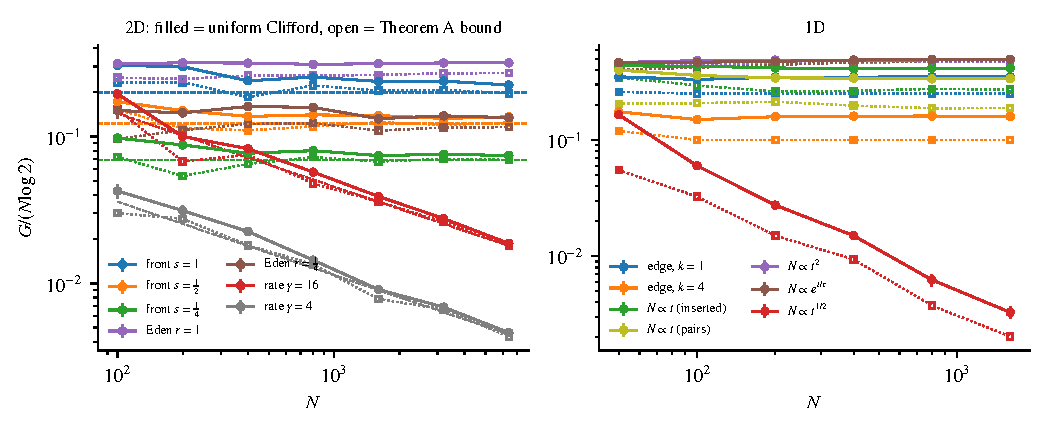
\includegraphics[width=\textwidth]{figures/fig_dichotomy.pdf}
\caption{Deficit per degree of freedom, uniform Clifford. Filled symbols: simulation. Open symbols: bound of Theorem~A computed exactly for each realisation. Dashed (2D): analytic predictions $f_2(2/s)/2$ and $\gamma R/(2\pi N)$. Left (2D): fronts and Eden keep a constant $G/N$, whereas the constant rate decreases like $N^{-1/2}$. Right (1D): decelerated insertion is the only class that tends to~$0$.}
\label{fig:dichotomy}
\end{figure}

\begin{itemize}[leftmargin=*,itemsep=1pt]
\item \emph{Fronts and Eden}: the deficit is extensive, and $G/N$ is stable to a few per cent between $N=1600$ and $6400$. At $N=6400$ the measured bound agrees with $f_2(\lambda)/2$ to better than $2\,\%$, with no fitted parameter. The random circuit nearly reaches the bound: $G/G_{\rm LB}$ is $1.07$ to $1.17$, so the strict cone captures $85$ to $93\,\%$ of the observed deficit.
\item \emph{Constant rate}: $G/N$ decreases by a factor $\approx2$ for each quadrupling of $N$. The exponent of $G$ is $0.468(4)$ and $0.512(14)$, inside the pre-registered interval $[0.3,0.75]$. A constant global rate does not produce an extensive arrow in dimension~2.
\item \emph{Scaling laws} (Figure~\ref{fig:scaling}): between $N=1600$ and $6400$ the local exponent of $S$ is $0.82$ and $0.85$ for the $t^2$ fronts (bounds $0.84$ and $0.87$). These values are sub-volume, but still above the asymptotic value $\frac34$. The exponent is $0.66$ for the slow exponential front (bound $0.72$). The fast exponential front ($H=1$ per round) \emph{fails} as a test: no gate crosses the cut between $N=1600$ and $6400$, because growth is faster than the gate cadence. The criterion used to choose this parameter omitted this condition.
\end{itemize}

\begin{figure}[t]
\centering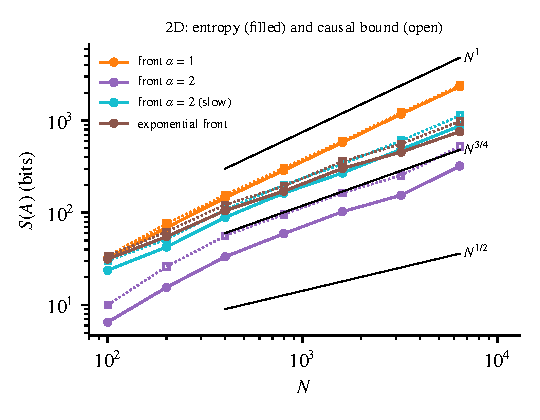
\includegraphics[width=0.5\textwidth]{figures/fig_scaling.pdf}
\caption{Entropy of one half (filled symbols) and causal bound (open symbols) in 2D, uniform Clifford. The linear front follows a volume law. The accelerated fronts ($R=at^2$) are clearly sub-volume, in their pre-asymptotic regime.}
\label{fig:scaling}
\end{figure}
